\begin{flushleft}
	{\color{blue!50!green}\fbox{\fontfamily{qag}\bfseries\selectfont PHẦN I. Câu trắc nghiệm nhiều phương án lựa chọn}}
	\textit{\small (Thí sinh trả lời từ câu 1 đến câu 12. Mỗi câu hỏi thí sinh chỉ chọn một phương án.)}
\end{flushleft}
\setcounter{ex}{0}
\setcounter{bt}{0}

% Câu 1
\begin{ex}
	\immini{\macau{ID: TOAN12-BT3-0103-C01}
		Cho hàm số bậc ba $y = f(x)$ có đồ thị như hình bên. Hàm số nghịch biến trên khoảng nào sau đây?
		\choice
		{$(-\infty; -1)$}
		{$(1; +\infty)$}
		{\True $(-1; 1)$}
		{$(-\infty; 1)$}
	}{
		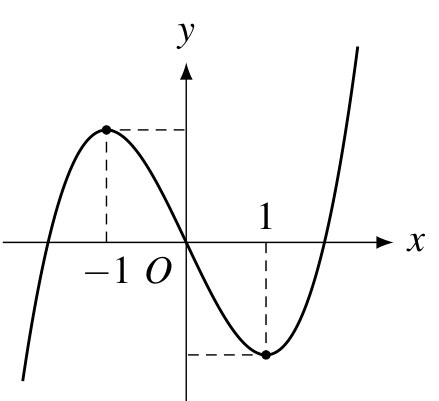
\includegraphics[width=3.6cm]{c1_hinh.png}
	}
	\loigiai{
		Dựa vào đồ thị hàm số, trên khoảng $(-1; 1)$ nét đồ thị đi xuống từ cực đại $(-1; 2)$ đến cực tiểu $(1; -2)$, do đó hàm số nghịch biến trên khoảng $(-1; 1)$.
	}
\end{ex}

% Câu 2
\begin{ex}
	\macau{ID: TOAN12-BT3-0103-C02}Cho hàm số $y = f(x)$ có bảng biến thiên như dưới đây:
	\begin{center}
	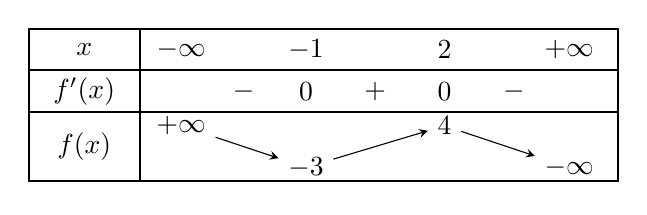
\begin{tikzpicture}[>=stealth,scale=0.88]
	  \draw[thick] (0,0) rectangle (8.5,-2.2);
	  \draw[thick] (0,-0.6) -- (8.5,-0.6);
	  \draw[thick] (0,-1.2) -- (8.5,-1.2);
	  \draw[thick] (1.6,0) -- (1.6,-2.2);
	  \node at (0.8,-0.3) {$x$};
	  \node at (0.8,-0.9) {$f'(x)$};
	  \node at (0.8,-1.7) {$f(x)$};
	  \node at (2.2,-0.3) {$-\infty$};
	  \node at (4.0,-0.3) {$-1$};
	  \node at (6.0,-0.3) {$2$};
	  \node at (7.8,-0.3) {$+\infty$};
	  \node at (3.1,-0.9) {$-$};
	  \node at (4.0,-0.9) {$0$};
	  \node at (5.0,-0.9) {$+$};
	  \node at (6.0,-0.9) {$0$};
	  \node at (7.0,-0.9) {$-$};
	  \node (p1) at (2.2,-1.4) {$+\infty$};
	  \node (p2) at (4.0,-2.0) {$-3$};
	  \node (p3) at (6.0,-1.4) {$4$};
	  \node (p4) at (7.8,-2.0) {$-\infty$};
	  \draw[->] (p1) -- (p2);
	  \draw[->] (p2) -- (p3);
	  \draw[->] (p3) -- (p4);
	\end{tikzpicture}
	\end{center}
	Giá trị cực tiểu của hàm số là
	\choice
	{\True $-3$}
	{$-1$}
	{$2$}
	{$4$}
	\loigiai{
		Từ bảng biến thiên, khi qua $x = -1$, đạo hàm $f'(x)$ đổi dấu từ âm sang dương nên hàm số đạt cực tiểu tại $x = -1$ và giá trị cực tiểu của hàm số là $y_{\text{CT}} = -3$.
	}
\end{ex}

% Câu 3
\begin{ex}
	\macau{ID: TOAN12-BT3-0103-C03}Cho hàm số $y = \dfrac{x - 4}{2x + 1}$. Tâm đối xứng của đồ thị là
	\choice
	{$I\left(-\dfrac{1}{2}; -\dfrac{1}{2}\right)$}
	{$I\left(\dfrac{1}{2}; -\dfrac{1}{2}\right)$}
	{$I(2; 1)$}
	{\True $I\left(-\dfrac{1}{2}; \dfrac{1}{2}\right)$}
	\loigiai{
		Đồ thị hàm số phân thức bậc nhất trên bậc nhất có tiệm cận đứng $x = -\dfrac{1}{2}$ và tiệm cận ngang $y = \dfrac{1}{2}$. Tâm đối xứng của đồ thị là giao điểm hai tiệm cận: $I\left(-\dfrac{1}{2}; \dfrac{1}{2}\right)$.
	}
\end{ex}

\newpage
% Câu 4
\begin{ex}
	\macau{ID: TOAN12-BT3-0103-C04}Cho hàm số $y = \dfrac{2x + 5}{x + 1}$. Khẳng định nào sau đây đúng?
	\choice
	{Hàm số đồng biến trên từng khoảng xác định}
	{\True Hàm số nghịch biến trên từng khoảng xác định}
	{Hàm số có một điểm cực trị}
	{Đồ thị không có tiệm cận ngang}
	\loigiai{
		Tập xác định $D = \mathbb{R} \setminus \{-1\}$. Ta có đạo hàm $y' = \dfrac{2(1) - 5(1)}{(x + 1)^2} = \dfrac{-3}{(x + 1)^2} < 0, \; \forall x \ne -1$. Vậy hàm số nghịch biến trên từng khoảng xác định $(-\infty; -1)$ và $(-1; +\infty)$.
	}
\end{ex}

% Câu 5
\begin{ex}
	\macau{ID: TOAN12-BT3-0103-C05}Cho hàm số $y = x + \dfrac{1}{x}$. Phương trình đường tiệm cận xiên của đồ thị hàm số là
	\choice
	{\True $y = x$}
	{$y = x + 1$}
	{$y = x - 1$}
	{$x = 0$}
	\loigiai{
		Ta có $\lim\limits_{x \to \pm\infty} [y - x] = \lim\limits_{x \to \pm\infty} \dfrac{1}{x} = 0$, do đó đường thẳng $y = x$ là đường tiệm cận xiên của đồ thị hàm số.
	}
\end{ex}

% Câu 6
\begin{ex}
	\macau{ID: TOAN12-BT3-0103-C06}Cho hàm số $y = x + 1 + \dfrac{2}{x + 1}$. Giao điểm hai đường tiệm cận của đồ thị hàm số là
	\choice
	{$I(1; 2)$}
	{$I(-1; 1)$}
	{\True $I(-1; 0)$}
	{$I(0; -1)$}
	\loigiai{
		Đồ thị hàm số có tiệm cận đứng $x = -1$ và tiệm cận xiên $y = x + 1$. Thay $x = -1$ vào phương trình tiệm cận xiên ta được $y = -1 + 1 = 0$. Vậy giao điểm hai tiệm cận là $I(-1; 0)$.
	}
\end{ex}

% Câu 7
\begin{ex}
	\macau{ID: TOAN12-BT3-0103-C07}Cho hàm số $y = f(x)$ có đạo hàm $f'(x) = 3(x - 1)(x + 3)$ với mọi $x \in \mathbb{R}$. Điểm cực đại của hàm số đã cho là
	\choice
	{$x = 1$}
	{\True $x = -3$}
	{$x = 3$}
	{$x = -1$}
	\loigiai{
		Phương trình $f'(x) = 0 \iff x = 1$ hoặc $x = -3$. Qua $x = -3$, đạo hàm $f'(x)$ đổi dấu từ dương sang âm, do đó hàm số đạt cực đại tại $x = -3$.
	}
\end{ex}

% Câu 8
\begin{ex}
	\macau{ID: TOAN12-BT3-0103-C08}Cho hàm số $y = f(x) = x^3 + 6x^2 + 9x$. Tâm đối xứng của đồ thị là
	\choice
	{$I(-1; 0)$}
	{$I(2; -2)$}
	{$I(-2; 0)$}
	{\True $I(-2; -2)$}
	\loigiai{
		Ta có $y' = 3x^2 + 12x + 9 \implies y'' = 6x + 12 = 0 \iff x = -2 \implies y(-2) = -2$. Tâm đối xứng của đồ thị hàm số bậc ba là điểm uốn $I(-2; -2)$.
	}
\end{ex}

\newpage
% Câu 9
\begin{ex}
	\macau{ID: TOAN12-BT3-0103-C09}Cho hàm số $y = f(x)$ có đạo hàm $f'(x) = x(x - 1)(x + 2)$ với mọi $x \in \mathbb{R}$. Số khoảng đồng biến của hàm số là
	\choice
	{$1$}
	{$3$}
	{\True $2$}
	{$4$}
	\loigiai{
		Phương trình $f'(x) = 0 \iff x \in \{-2; 0; 1\}$. Xét dấu $f'(x)$, ta thấy $f'(x) > 0$ trên $(-2; 0)$ và $(1; +\infty)$. Vậy hàm số có đúng 2 khoảng đồng biến.
	}
\end{ex}

% Câu 10
\begin{ex}
	\macau{ID: TOAN12-BT3-0103-C10}Cho hàm số $y = \dfrac{ax^2 + bx + c}{dx + e}$ ($ad \ne 0$), trong đó đa thức tử không chia hết cho đa thức mẫu. Bảng biến thiên của hàm số được cho như dưới đây:
	\begin{center}
	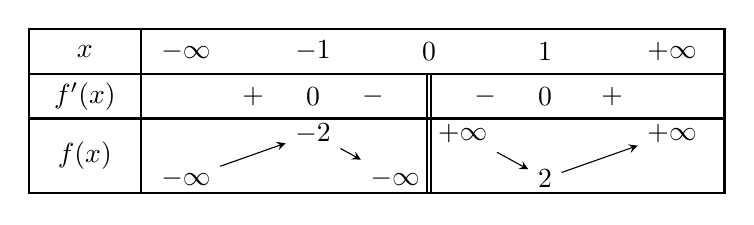
\begin{tikzpicture}[>=stealth,scale=0.95]
	  \draw[thick] (0,0) rectangle (9.3,-2.2);
	  \draw[thick] (0,-0.6) -- (9.3,-0.6);
	  \draw[thick] (0,-1.2) -- (9.3,-1.2);
	  \draw[thick] (1.5,0) -- (1.5,-2.2);
	  \draw[thick] (5.32,-0.6) -- (5.32,-2.2);
	  \draw[thick] (5.38,-0.6) -- (5.38,-2.2);
	  \node at (0.75,-0.3) {$x$};
	  \node at (0.75,-0.9) {$f'(x)$};
	  \node at (0.75,-1.7) {$f(x)$};
	  \node at (2.1,-0.3) {$-\infty$};
	  \node at (3.8,-0.3) {$-1$};
	  \node at (5.35,-0.3) {$0$};
	  \node at (6.9,-0.3) {$1$};
	  \node at (8.6,-0.3) {$+\infty$};
	  \node at (3.0,-0.9) {$+$};
	  \node at (3.8,-0.9) {$0$};
	  \node at (4.6,-0.9) {$-$};
	  \node at (6.1,-0.9) {$-$};
	  \node at (6.9,-0.9) {$0$};
	  \node at (7.8,-0.9) {$+$};
	  \node (p1) at (2.1,-2.0) {$-\infty$};
	  \node (p2) at (3.8,-1.4) {$-2$};
	  \node (p3) at (4.9,-2.0) {$-\infty$};
	  \node (p4) at (5.8,-1.4) {$+\infty$};
	  \node (p5) at (6.9,-2.0) {$2$};
	  \node (p6) at (8.6,-1.4) {$+\infty$};
	  \draw[->] (p1) -- (p2);
	  \draw[->] (p2) -- (p3);
	  \draw[->] (p4) -- (p5);
	  \draw[->] (p5) -- (p6);
	\end{tikzpicture}
	\end{center}
	Hàm số nào dưới đây có bảng biến thiên đã cho?
	\choice
	{\True $y = \dfrac{x^2 + 1}{x}$}
	{$y = \dfrac{x^2 - 1}{x}$}
	{$y = \dfrac{x^2 + 1}{x - 1}$}
	{$y = \dfrac{x^2 + 4}{x}$}
	\loigiai{
		Từ bảng biến thiên, đồ thị có tiệm cận đứng $x = 0$, điểm cực đại $(-1; -2)$ và cực tiểu $(1; 2)$. Hàm số $y = \dfrac{x^2 + 1}{x} = x + \dfrac{1}{x}$ có tiệm cận đứng $x = 0$, đạo hàm $y' = \dfrac{x^2 - 1}{x^2} = 0 \iff x = \pm 1$, cực đại $(-1; -2)$ và cực tiểu $(1; 2)$, hoàn toàn phù hợp.
	}
\end{ex}

% Câu 11
\begin{ex}
	\macau{ID: TOAN12-BT3-0103-C11}Cho hàm số $y = x + 2 + \dfrac{3}{x - 2}$. Phương trình đường tiệm cận xiên của đồ thị hàm số là
	\choice
	{$x = 2$}
	{$y = 2$}
	{\True $y = x + 2$}
	{$y = x - 2$}
	\loigiai{
		Vì $\lim\limits_{x \to \pm\infty} [y - (x + 2)] = \lim\limits_{x \to \pm\infty} \dfrac{3}{x - 2} = 0$, nên đường thẳng $y = x + 2$ là đường tiệm cận xiên của đồ thị hàm số.
	}
\end{ex}

% Câu 12
\begin{ex}
	\macau{ID: TOAN12-BT3-0103-C12}Cho hàm số $y = f(x)$ xác định trên $\mathbb{R} \setminus \{-1\}$ và có đạo hàm $f'(x) = \dfrac{x(x + 2)}{(x + 1)^2}$. Điểm cực đại của hàm số đã cho là
	\choice
	{$x = -1$}
	{$x = 0$}
	{$x = 2$}
	{\True $x = -2$}
	\loigiai{
		Vì $(x + 1)^2 > 0$ với mọi $x \ne -1$ nên dấu của $f'(x)$ cùng dấu với $x(x + 2)$. Khi qua $x = -2$, $f'(x)$ đổi dấu từ dương sang âm, do đó hàm số đạt cực đại tại $x = -2$.
	}
\end{ex}

\newpage
\begin{flushleft}
	{\color{blue!50!green}\fbox{\fontfamily{qag}\bfseries\selectfont PHẦN II. Câu trắc nghiệm đúng sai}}
	\textit{\small (Thí sinh trả lời từ câu 1 đến câu 4. Trong mỗi ý a), b), c), d) ở mỗi câu, thí sinh chọn đúng hoặc sai.)}
\end{flushleft}
\setcounter{ex}{0}
\setcounter{bt}{0}

% Phần II Câu 1
\begin{ex}
	\immini{\macau{ID: TOAN12-BT3-0103-C13}
		Cho hàm số $y = \dfrac{2x + 1}{x - 1}$. Xét tính đúng, sai của các phát biểu sau:
		\choiceTF
		{\True Đạo hàm của hàm số là $y' = -\dfrac{3}{(x - 1)^2}$}
		{Hàm số đồng biến trên khoảng $(1; +\infty)$}
		{\True Đồ thị có tiệm cận ngang $y = 2$}
		{Hình bên là đồ thị của hàm số đã cho}
	}{
		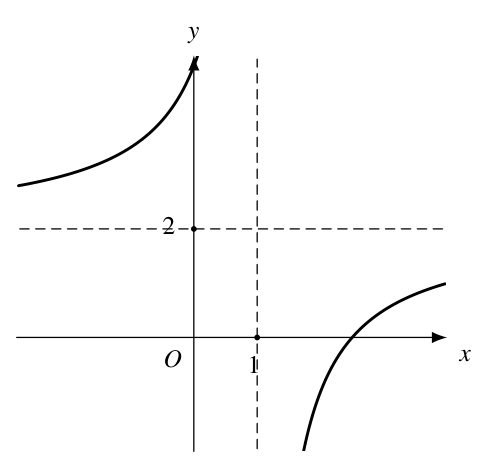
\includegraphics[width=4.0cm]{p2_c1_hinh.png}
	}
	\loigiai{
		a) \textbf{Đúng}: $y' = \dfrac{2(-1) - 1(1)}{(x - 1)^2} = -\dfrac{3}{(x - 1)^2} < 0, \; \forall x \ne 1$.\\
		b) \textbf{Sai}: Vì $y' < 0$ trên $(1; +\infty)$ nên hàm số nghịch biến trên khoảng $(1; +\infty)$.\\
		c) \textbf{Đúng}: $\lim\limits_{x \to \pm\infty} y = 2$ nên tiệm cận ngang là $y = 2$.\\
		d) \textbf{Sai}: Với $x > 1$ thì $y = 2 + \dfrac{3}{x - 1} > 2$, nhánh đồ thị bên phải phải nằm trên đường $y = 2$, trong khi hình vẽ hiển thị nhánh bên phải nằm dưới đường $y = 2$.
	}
\end{ex}

% Phần II Câu 2
\begin{ex}
	\immini{\macau{ID: TOAN12-BT3-0103-C14}
		Cho hàm số $y = \dfrac{ax^2 + bx + c}{dx + e}$ ($ad \ne 0$), trong đó đa thức tử không chia hết cho đa thức mẫu. Đồ thị của hàm số được cho như hình bên. Xét tính đúng, sai của các phát biểu sau:
		\choiceTF
		{\True Đồ thị có tiệm cận đứng $x = 1$}
		{\True Đường tiệm cận xiên có phương trình $y = x + 2$}
		{Đồ thị cắt trục tung tại điểm có tung độ bằng $2$}
		{Hàm số nghịch biến trên toàn bộ $\mathbb{R}$}
	}{
		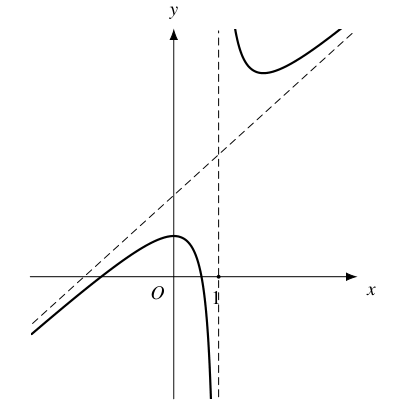
\includegraphics[width=3.8cm]{p2_c2_hinh.png}
	}
	\loigiai{
		a) \textbf{Đúng}: Đồ thị có đường tiệm cận đứng là $x = 1$.\\
		b) \textbf{Đúng}: Tiệm cận xiên đi qua $(0; 2)$ và $(-2; 0)$, có phương trình $y = x + 2$.\\
		c) \textbf{Sai}: Đồ thị cắt trục tung tại điểm cực đại $(0; 1)$, tung độ bằng $1 \ne 2$.\\
		d) \textbf{Sai}: Hàm số không xác định tại $x = 1$, không thể nghịch biến trên toàn bộ $\mathbb{R}$.
	}
\end{ex}

\newpage
% Phần II Câu 3
\begin{ex}
	\macau{ID: TOAN12-BT3-0103-C15}Cho hàm số $y = \dfrac{(x - 2)^2}{x - 1}$. Xét tính đúng, sai của các phát biểu sau:
	\choiceTF
	{\True Tập xác định của hàm số là $\mathbb{R} \setminus \{1\}$}
	{Hàm số nghịch biến trên khoảng $(-\infty; 0)$}
	{Hàm số đạt cực tiểu tại $x = 0$}
	{\True Đồ thị có tiệm cận xiên $y = x - 3$}
	\loigiai{
		Ta có $y = \dfrac{x^2 - 4x + 4}{x - 1} = x - 3 + \dfrac{1}{x - 1}$ và $y' = \dfrac{x(x - 2)}{(x - 1)^2}$.\\
		a) \textbf{Đúng}: Điều kiện xác định $x \ne 1 \implies D = \mathbb{R} \setminus \{1\}$.\\
		b) \textbf{Sai}: Với $x \in (-\infty; 0)$, $x(x - 2) > 0 \implies y' > 0$, hàm số đồng biến trên khoảng $(-\infty; 0)$.\\
		c) \textbf{Sai}: Qua $x = 0$, $y'$ đổi dấu từ dương sang âm nên $x = 0$ là điểm cực đại.\\
		d) \textbf{Đúng}: $\lim\limits_{x \to \pm\infty} [y - (x - 3)] = 0 \implies$ tiệm cận xiên là $y = x - 3$.
	}
\end{ex}

% Phần II Câu 4
\begin{ex}
	\macau{ID: TOAN12-BT3-0103-C16}Cho hàm số $y = f(x) = -x^3 + 3x + 1$. Xét tính đúng, sai của các phát biểu sau:
	\choiceTF
	{\True Đạo hàm của hàm số là $f'(x) = 3(1 - x^2)$}
	{\True Hàm số đồng biến trên khoảng $(-1; 1)$}
	{Giá trị cực tiểu của hàm số bằng $1$}
	{\True Bảng biến thiên dưới đây là bảng biến thiên của hàm số đã cho
		\begin{center}
		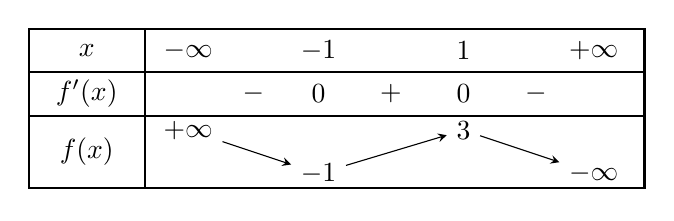
\begin{tikzpicture}[>=stealth,scale=0.92]
		  \draw[thick] (0,0) rectangle (8.5,-2.2);
		  \draw[thick] (0,-0.6) -- (8.5,-0.6);
		  \draw[thick] (0,-1.2) -- (8.5,-1.2);
		  \draw[thick] (1.6,0) -- (1.6,-2.2);
		  \node at (0.8,-0.3) {$x$};
		  \node at (0.8,-0.9) {$f'(x)$};
		  \node at (0.8,-1.7) {$f(x)$};
		  \node at (2.2,-0.3) {$-\infty$};
		  \node at (4.0,-0.3) {$-1$};
		  \node at (6.0,-0.3) {$1$};
		  \node at (7.8,-0.3) {$+\infty$};
		  \node at (3.1,-0.9) {$-$};
		  \node at (4.0,-0.9) {$0$};
		  \node at (5.0,-0.9) {$+$};
		  \node at (6.0,-0.9) {$0$};
		  \node at (7.0,-0.9) {$-$};
		  \node (p1) at (2.2,-1.4) {$+\infty$};
		  \node (p2) at (4.0,-2.0) {$-1$};
		  \node (p3) at (6.0,-1.4) {$3$};
		  \node (p4) at (7.8,-2.0) {$-\infty$};
		  \draw[->] (p1) -- (p2);
		  \draw[->] (p2) -- (p3);
		  \draw[->] (p3) -- (p4);
		\end{tikzpicture}
		\end{center}
	}
	\loigiai{
		a) \textbf{Đúng}: $f'(x) = -3x^2 + 3 = 3(1 - x^2)$.\\
		b) \textbf{Đúng}: Trên khoảng $(-1; 1)$, $1 - x^2 > 0 \implies f'(x) > 0$, hàm số đồng biến.\\
		c) \textbf{Sai}: Tại $x = -1$, giá trị cực tiểu là $f(-1) = -1 \ne 1$.\\
		d) \textbf{Đúng}: Bảng biến thiên thể hiện đúng chiều biến thiên và các giá trị cực trị $y_{\text{CT}} = -1$, $y_{\text{CĐ}} = 3$.
	}
\end{ex}

\newpage
\begin{flushleft}
	{\color{blue!50!green}\fbox{\fontfamily{qag}\bfseries\selectfont PHẦN III. Câu trắc nghiệm yêu cầu trả lời ngắn}}
	\textit{\small (Thí sinh trả lời từ câu 1 đến câu 6.)}
\end{flushleft}
\setcounter{ex}{0}
\setcounter{bt}{0}

% Phần III Câu 1
\begin{ex}
	\macau{ID: TOAN12-BT3-0103-C17}Cho hàm số $y = f(x)$ có bảng biến thiên như dưới đây:
	\begin{center}
	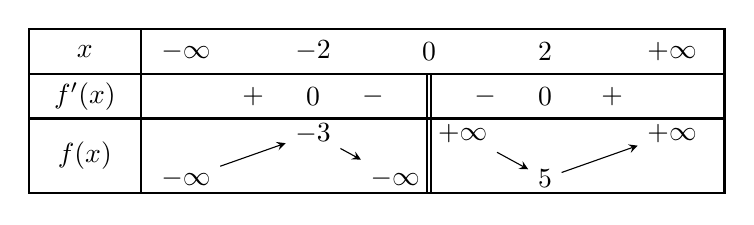
\begin{tikzpicture}[>=stealth,scale=0.95]
	  \draw[thick] (0,0) rectangle (9.3,-2.2);
	  \draw[thick] (0,-0.6) -- (9.3,-0.6);
	  \draw[thick] (0,-1.2) -- (9.3,-1.2);
	  \draw[thick] (1.5,0) -- (1.5,-2.2);
	  \draw[thick] (5.32,-0.6) -- (5.32,-2.2);
	  \draw[thick] (5.38,-0.6) -- (5.38,-2.2);
	  \node at (0.75,-0.3) {$x$};
	  \node at (0.75,-0.9) {$f'(x)$};
	  \node at (0.75,-1.7) {$f(x)$};
	  \node at (2.1,-0.3) {$-\infty$};
	  \node at (3.8,-0.3) {$-2$};
	  \node at (5.35,-0.3) {$0$};
	  \node at (6.9,-0.3) {$2$};
	  \node at (8.6,-0.3) {$+\infty$};
	  \node at (3.0,-0.9) {$+$};
	  \node at (3.8,-0.9) {$0$};
	  \node at (4.6,-0.9) {$-$};
	  \node at (6.1,-0.9) {$-$};
	  \node at (6.9,-0.9) {$0$};
	  \node at (7.8,-0.9) {$+$};
	  \node (p1) at (2.1,-2.0) {$-\infty$};
	  \node (p2) at (3.8,-1.4) {$-3$};
	  \node (p3) at (4.9,-2.0) {$-\infty$};
	  \node (p4) at (5.8,-1.4) {$+\infty$};
	  \node (p5) at (6.9,-2.0) {$5$};
	  \node (p6) at (8.6,-1.4) {$+\infty$};
	  \draw[->] (p1) -- (p2);
	  \draw[->] (p2) -- (p3);
	  \draw[->] (p4) -- (p5);
	  \draw[->] (p5) -- (p6);
	\end{tikzpicture}
	\end{center}
	Hàm số có bao nhiêu điểm cực trị?
	\par\shortans[oly]{2}
	\loigiai{
		Qua $x = -2$, $f'(x)$ đổi dấu từ dương sang âm nên $x = -2$ là điểm cực đại. Qua $x = 2$, $f'(x)$ đổi dấu từ âm sang dương nên $x = 2$ là điểm cực tiểu. Tại $x = 0$, hàm số không xác định nên không là điểm cực trị. Vậy hàm số có đúng $2$ điểm cực trị.
	}
\end{ex}

% Phần III Câu 2
\begin{ex}
	\macau{ID: TOAN12-BT3-0103-C18}Cho hàm số $y = f(x) = x^3 - 6x^2 + 9x + 1$. Tính hiệu giữa giá trị cực đại và giá trị cực tiểu của hàm số.
	\par\shortans[oly]{4}
	\loigiai{
		Ta có $f'(x) = 3x^2 - 12x + 9 = 3(x - 1)(x - 3) = 0 \iff x = 1$ hoặc $x = 3$.\\
		Giá trị cực đại $y_{\text{CĐ}} = f(1) = 5$, giá trị cực tiểu $y_{\text{CT}} = f(3) = 1$.\\
		Hiệu giữa giá trị cực đại và giá trị cực tiểu là: $y_{\text{CĐ}} - y_{\text{CT}} = 5 - 1 = 4$.
	}
\end{ex}

% Phần III Câu 3
\begin{ex}
	\macau{ID: TOAN12-BT3-0103-C19}Cho hàm số $y = \dfrac{2x + 1}{x - 1}$. Gọi $I(a; b)$ là giao điểm hai đường tiệm cận. Tính $a + b$.
	\par\shortans[oly]{3}
	\loigiai{
		Đồ thị có tiệm cận đứng $x = 1$ và tiệm cận ngang $y = 2$. Giao điểm hai đường tiệm cận là $I(1; 2)$, suy ra $a = 1, b = 2$. Vậy $a + b = 1 + 2 = 3$.
	}
\end{ex}

\newpage
% Phần III Câu 4
\begin{ex}
	\macau{ID: TOAN12-BT3-0103-C20}Cho hàm số $y = \dfrac{x^2 - 1}{x - 2}$. Tính tung độ giao điểm của đường tiệm cận xiên của đồ thị với trục tung.
	\par\shortans[oly]{2}
	\loigiai{
		Thực hiện phép chia: $y = \dfrac{x^2 - 1}{x - 2} = x + 2 + \dfrac{3}{x - 2}$.\\
		Đường tiệm cận xiên của đồ thị là $y = x + 2$. Cho $x = 0$ ta được $y = 2$. Vậy tung độ giao điểm của đường tiệm cận xiên với trục tung là $2$.
	}
\end{ex}

% Phần III Câu 5
\begin{ex}
	\macau{ID: TOAN12-BT3-0103-C21}Cho hàm số $y = f(x)$ có đạo hàm $f'(x) = (x + 3)(x - 1)^2(x - 2)$ với mọi $x \in \mathbb{R}$. Tính tổng các giá trị của $x$ tại đó hàm số đạt cực trị.
	\par\shortans[oly]{-1}
	\loigiai{
		Phương trình $f'(x) = 0$ có hai nghiệm đơn $x = -3$, $x = 2$ và một nghiệm bội hai $x = 1$. Đạo hàm $f'(x)$ chỉ đổi dấu qua các nghiệm đơn $x = -3$ và $x = 2$. Do đó hàm số đạt cực trị tại $x_1 = -3$ và $x_2 = 2$. Tổng các giá trị cực trị là: $(-3) + 2 = -1$.
	}
\end{ex}

% Câu 6
\begin{ex}
	\macau{ID: TOAN12-BT3-0103-C22}Cho hàm số $y = f(x) = x^3 - 3ax$, với $a > 0$. Biết hàm số đạt cực tiểu tại $x = 3$. Tính $a$.
	\par\shortans[oly]{9}
	\loigiai{
		Ta có $f'(x) = 3(x^2 - a) = 0 \iff x = \pm\sqrt{a}$ (do $a > 0$). Vì $f''(x) = 6x \implies f''(\sqrt{a}) = 6\sqrt{a} > 0$ nên hàm số đạt cực tiểu tại $x = \sqrt{a}$. Theo giả thiết hàm số đạt cực tiểu tại $x = 3$, suy ra $\sqrt{a} = 3 \iff a = 9$.
	}
\end{ex}
